\documentclass[18pt]{article}
\usepackage[utf8]{inputenc}
\usepackage[T1]{fontenc}
\usepackage{ragged2e}
\usepackage{caladea}
\usepackage{graphicx}
\usepackage{longtable}
\usepackage{wrapfig}
\usepackage{rotating}
\usepackage{epigraph}
\usepackage[normalem]{ulem}
\usepackage{hyperref}
\usepackage{amsmath}
\usepackage{amssymb}
\usepackage{capt-of}
\usepackage{hyperref}
\usepackage{fancyhdr}

\title{
 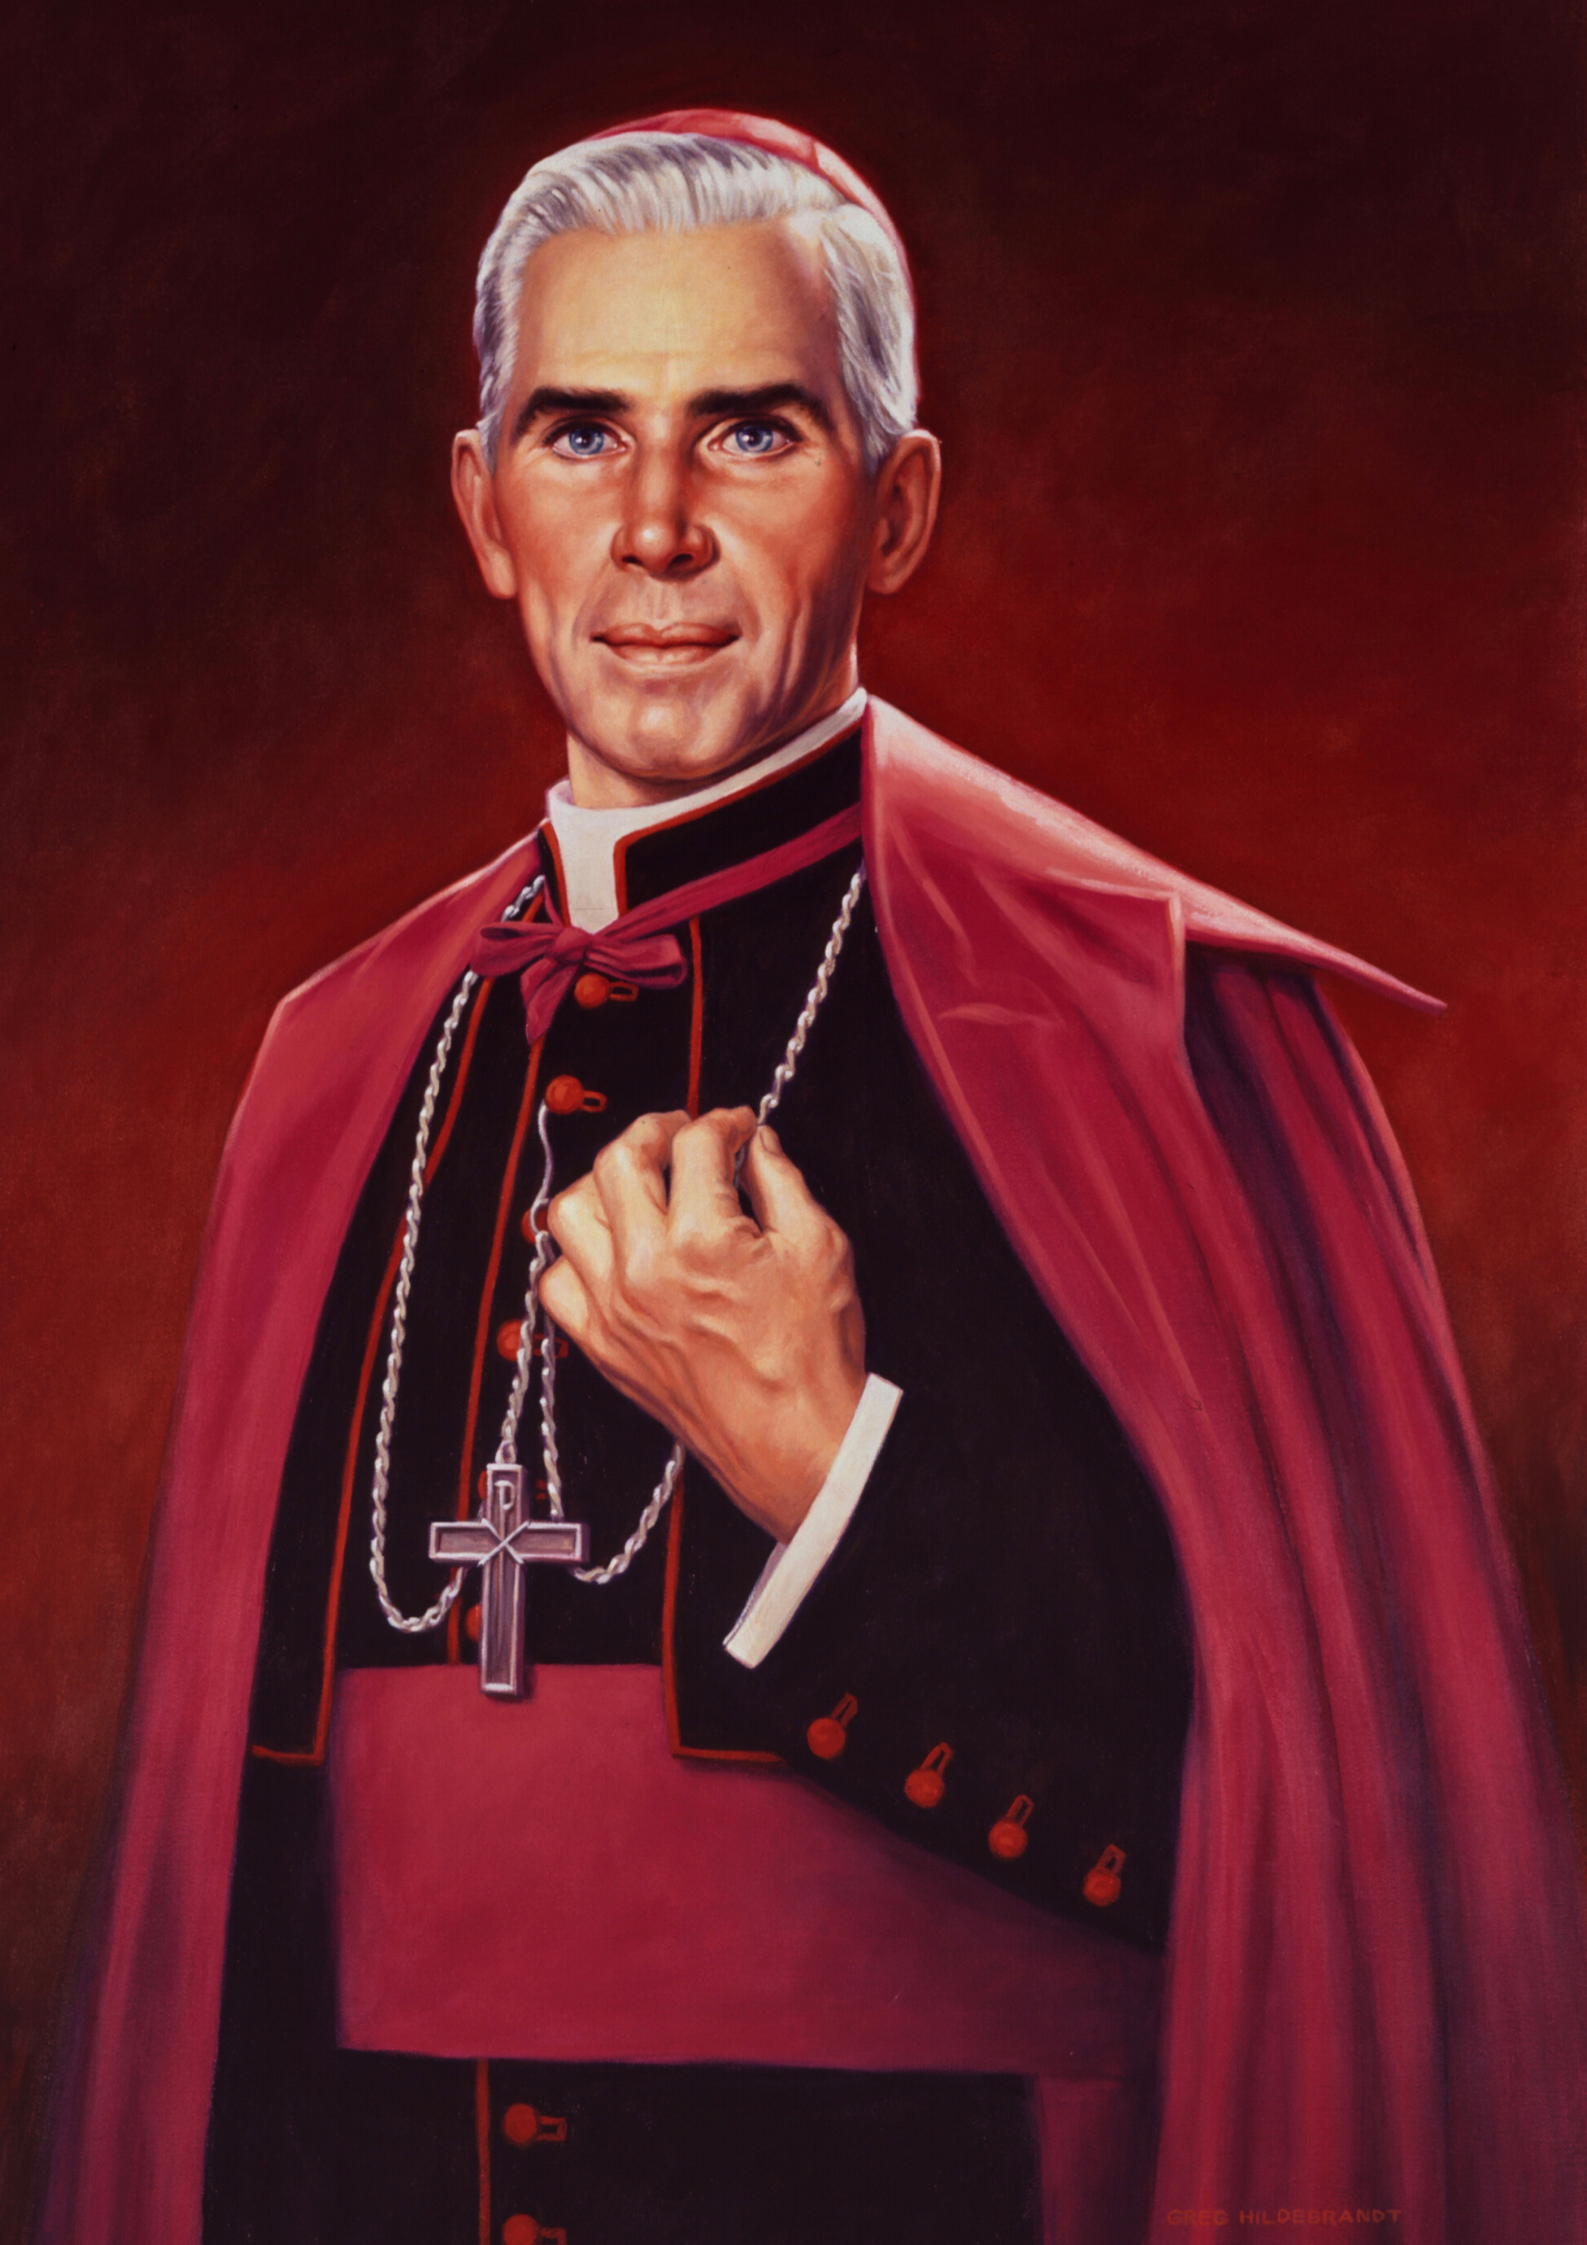
\includegraphics[scale=0.25, trim={10cm, 0, 10cm, 0}]{./assets/imagem.jpg}
  \par
   NOVENA AO NAZARENO NEGRO}
\author{Garamog, Nina Freitas}
\date{Início da Novena: 31/12 - Data Litúrgica: 09/01 }

% Comando para fazer "Sumário" não aparecer no Sumário.
\renewcommand{\contentsname}{Sumário}
\begin{document}
\maketitle

\thispagestyle{empty} %zera a primeira página

\pagestyle{fancy}
\fancyhf{} % clear existing header/footer entries
\fancyfoot[LO, CE]{
  \includegraphics[scale=0.2]{./assets/cross.png} Nazareno Negro, cuidai de nós!
}
% Place Page X of Y on the right-hand
% side of the footer
\fancyfoot[R]{\thepage}

\newpage

\tableofcontents

\centering
\vfill
Visite-nos no Telegram: \url{https://t.me/CotidieNovena}
\newpage

\newpage


\begin{justify}

 \begin{center}
  \section{História}\label{sec:História} % (fold)
 \end{center}


\subsection{Sobre o Nazareno Negro}\label{sub:Sobre o Nazareno Negro} % (fold)
 
\hspace{.45cm} O Nazareno Negro é uma imagem de Jesus. Foi esculpida por um artista mexicano desconhecido no século XVI e atualmente está consagrada nas Filipinas.

Muitos milagres têm sido atribuídos à veneração da imagem do Nazareno Negro. Você pode usar esta novena para buscar ajuda de Jesus sob o título do Nazareno Negro em sua própria vida!

 % subsection Sobre o Nazareno Negro (end)


\subsection{Chegada da Imagem às Filipinas}

\hspace{.45cm} Em 1606, um grupo de missionários agostinianos viajou do México para as Filipinas. Eles levaram a imagem do Nazareno Negro com eles para Manila.


\subsection{Características da Imagem}

\hspace{.45cm} A imagem do Nazareno Negro é uma representação em tamanho real de Jesus com pele escura. Ela O mostra ajoelhado com um joelho no chão, sob Sua cruz. Ele é mostrado descalço e em agonia devido ao peso pesado da cruz. A cruz é feita de madeira preta, e as pontas dela são cobertas com tampas de latão.


\subsection{Detalhes Simbólicos da Imagem}

\hspace{.45cm} Na imagem, Jesus usa uma coroa de espinhos. A imagem O mostra com um halo "Tres Potencias" (ou "Três Potências") que tem vários significados simbólicos. 

\begin{itemize}
 \item \textbf{Santíssima Trindade:} Um dos significados do halo é a representação da Trindade.
 \item \textbf{Faculdades de Jesus:} Outro significado está relacionado às faculdades de vontade, memória e entendimento na alma de Jesus.
 \item \textbf{Autoridade e Força:} O halo também simboliza a autoridade, poder e força de Jesus.
\end{itemize}


\subsection{As Vestes do Nazareno Negro}

\hspace{.45cm} A imagem do Nazareno Negro está vestida com uma túnica de veludo bordô. A túnica é bordada com fios de ouro. Renda branca adorna o colarinho e os punhos da túnica. Um cinto dourado está ao redor da cintura, e a palavra "Nazareno" está gravada nele.

Para representar a flagelação, uma corrente dourada que termina em esferas está loopada ao redor do pescoço de Jesus e segurada em Sua mão esquerda. Em cinco ocasiões diferentes ao longo do ano, para preparar certas festas, as vestes da imagem são trocadas.


\subsection{A Cor Escura da Imagem}

\hspace{.45cm} Acredita-se que a cor escura da imagem venha da madeira de mesquite da qual foi esculpida.


\subsection{Aprovação Papal e Confraria}

\hspace{.45cm} Em 1650, o Papa Inocêncio X aprovou a veneração da imagem. Ele também reconheceu oficialmente a Confraria leiga de Santo Cristo Jesus Nazareno. Esta confraria promoveu a devoção a Jesus por meio da imagem do Nazareno Negro.


\subsection{Localização e Consagração da Imagem}

\hspace{.45cm} A imagem do Nazareno Negro foi primeiro consagrada na Igreja Agostiniana de São João Batista, em Luneta. Ela foi colocada em várias igrejas diferentes próximas a Manila até 1787, quando foi consagrada em Quiapo. Nas Filipinas, a imagem é amplamente venerada. Muitos milagres têm sido associados à veneração da imagem.


\subsection{Devoção Popular nas Filipinas}

\hspace{.45cm} A devoção ao Nazareno Negro continua sendo muito popular na cultura filipina. Muitos filipinos pobres uniram seus sofrimentos de pobreza aos sofrimentos da Paixão de Jesus por meio da devoção ao Nazareno Negro.


\subsection{A Procissão da Translacion}

\hspace{.45cm} Todo ano, na Festa do Nazareno Negro, uma procissão chamada *Translacion* leva muitos católicos até a Basílica de João Batista. Essa procissão reencena a transferência solene da imagem para seu atual local de residência na basílica.

A imagem também é levada em procissão todo ano na Sexta-feira Santa e na véspera de Ano Novo.


\end{justify}

%%%%%%%%%%%%%%%%%%%%%%%%%%%%%%%%%%%%% Orações  %%%%%%%%%%%%%%%%%%%%%%%%%%%%%%%%%%%%%%%%%%%

\newpage
\section{Orações}\label{sec:Orações} % (fold)
\subsection{Oração Incial}\label{sec:Oração_Inicial} % (fold)

Querido Senhor, agradecemos pelas muitas práticas espirituais e devoções que o Senhor deu à Sua Igreja para nossa salvação. Por favor, conceda graça a todas as pessoas através da devoção ao Nazareno Negro!

\subsection{Primeiro Dia}
\textbf{\nameref{sec:Oração_Inicial}}

Sua imagem mostra o Senhor carregando Sua cruz antes da Sua crucifixão. Podemos ver como o Senhor sofreu sob o peso da cruz por amor a nós. Através da contemplação de tudo o que o Senhor sofreu por nossa causa, podemos nos aproximar mais de Ti e cultivar uma amizade mais forte com o Senhor em nossas vidas.

Por favor, ouça todas as intenções que trazemos diante de Ti. E pedimos especialmente hoje que o Senhor nos ajude, a nós e a todas as pessoas, a crescer em uma amizade mais profunda com o Senhor!

Ajude-nos a tornar o nosso relacionamento contigo a nossa maior prioridade na vida. Dê-nos a graça de fazer tudo o que for necessário para nossa santidade.

\textbf{\nameref{sec:Oração_Final}}

\subsection{Segundo Dia}
\textbf{\nameref{sec:Oração_Inicial}}



O Senhor sofreu uma dor inimaginável por nossa causa. Sua imagem do Nazareno Negro retrata parte desse sofrimento para que possamos contemplá-lo. Podemos ver como o Senhor carregou a pesada cruz, como Sua cabeça foi dolorosamente perfurada por uma coroa de espinhos e como o Senhor foi cruelmente flagelado.

Por favor, ouça todas as intenções que trazemos diante de Ti. E pedimos especialmente hoje que o Senhor nos ajude, a nós e a todas as pessoas, a crescer em uma apreciação mais profunda de Seus sofrimentos!

Ajude-nos a crescer no amor pelo Senhor a cada dia de nossas vidas. Dê-nos a graça de entregar cada aspecto de nossas vidas ao Senhor.

\textbf{\nameref{sec:Oração_Final}}


\subsection{Terceiro Dia}
\textbf{\nameref{sec:Oração_Inicial}}




Sua imagem é venerada por muitas pessoas nas Filipinas. Existem muitas práticas piedosas associadas à veneração de Sua imagem. Através da veneração piedosa de Sua imagem e da confiança que os fiéis depositam em Ti, o Senhor realizou muitos milagres.

Por favor, ouça todas as intenções que trazemos diante de Ti. E pedimos especialmente hoje que o Senhor nos ajude, a nós e a todas as pessoas, a crescer em uma piedade mais profunda!

Ajude-nos a crescer em todas as virtudes necessárias para nossa santidade. Dê-nos a graça de fazer bom uso de toda ajuda que o Senhor nos deu para nossa salvação.

\textbf{\nameref{sec:Oração_Final}}


\subsection{Quarto Dia}
\textbf{\nameref{sec:Oração_Inicial}}

Sua imagem mostra o Senhor sofrendo sob o peso de Sua cruz, e nos lembra das muitas outras dores físicas que o Senhor suportou. Ao contemplarmos Sua Paixão e o grande sofrimento que o Senhor suportou, podemos crescer no santo desejo de sofrer com o Senhor em nossas vidas.

Por favor, ouça todas as intenções que trazemos diante de Ti. E pedimos especialmente hoje que o Senhor nos ajude, a nós e a todas as pessoas, a crescer no desejo de sofrer de maneira santa!

Ajude-nos a nos unir mais plenamente ao Senhor a cada dia de nossas vidas. Dê-nos a graça de oferecer todo sofrimento e as provações que enfrentamos em união com o Seu.

\textbf{\nameref{sec:Oração_Final}}


\subsection{Sexto Dia}
\textbf{\nameref{sec:Oração_Inicial}}




Muitas pessoas veneraram Sua imagem com grande devoção. O Senhor achou por bem conceder milagres em resposta a muitas orações feitas pelos fiéis enquanto veneravam Sua imagem. Sabemos que sempre podemos recorrer a Ti com fé para nossas próprias necessidades.

Por favor, ouça todas as intenções que trazemos diante de Ti. E pedimos especialmente hoje que o Senhor nos ajude, a nós e a todas as pessoas, a crescer na virtude da fé!

Ajude-nos a confiar na Sua bondade e providência em todos os aspectos de nossas vidas. Dê-nos a graça de nos entregarmos completamente ao Senhor em todas as circunstâncias.

\textbf{\nameref{sec:Oração_Final}}


\subsection{Quinto Dia}
\textbf{\nameref{sec:Oração_Inicial}}




Ao longo de nossas vidas na Terra, enfrentamos muitas provações e dificuldades. No meio do sofrimento, nem sempre é fácil lembrar de Seus santos sofrimentos e nos unir a Ti. A contemplação de Seus sofrimentos, retratados em Sua imagem, pode nos ajudar a unir nossos sofrimentos aos Seus de maneira mais perfeita.

Por favor, ouça todas as intenções que trazemos diante de Ti. E pedimos especialmente hoje que o Senhor nos ajude, a nós e a todas as pessoas, a crescer na capacidade de unir nossos sofrimentos aos Seus!

Ajude-nos a confiar em Ti para tudo o que precisamos em nossas vidas. Dê-nos a graça de abraçar toda provação que possamos enfrentar por amor a Ti.

\textbf{\nameref{sec:Oração_Final}}


\subsection{Sétimo Dia}
\textbf{\nameref{sec:Oração_Inicial}}




Sua imagem foi feita por um artista mexicano desconhecido. Depois, alguns membros da ordem religiosa agostiniana levaram Sua imagem para as Filipinas. Nas Filipinas, Sua imagem foi venerada por muitos católicos piedosos. O Senhor realizou inúmeros milagres para os fiéis que veneraram Sua imagem com piedade.

Por favor, ouça todas as intenções que trazemos diante de Ti. E pedimos especialmente hoje que o Senhor ajude todos os membros da ordem religiosa agostiniana a serem Seus servos santos!

Ajude-nos a amar o Senhor mais profundamente a cada dia de nossas vidas. Dê-nos a graça de fazer tudo o que pudermos para servi-Lo de maneira digna.

\textbf{\nameref{sec:Oração_Final}}


\subsection{Oitavo Dia}
\textbf{\nameref{sec:Oração_Inicial}}




Depois que Sua imagem foi levada para as Filipinas, muitos fiéis a veneraram através de práticas piedosas. Essa devoção deve ter sido agradável a Ti. O Senhor achou por bem conceder muitos milagres em resposta às orações dos fiéis que eram devotos de Ti.

Por favor, ouça todas as intenções que trazemos diante de Ti. E pedimos especialmente hoje que o Senhor abençoe todos aqueles que são devotos de Ti sob o título do Nazareno Negro!

Ajude-nos a fazer tudo o que pud

ermos para crescer em santidade a cada dia de nossas vidas. Dê-nos a graça de permitir que nosso amor pelo Senhor transforme completamente nossas vidas.

\textbf{\nameref{sec:Oração_Final}}

\subsection{Nono Dia}
\textbf{\nameref{sec:Oração_Inicial}}


Sua imagem foi levada para as Filipinas pelos agostinianos. Lá, a devoção ao Senhor através da veneração piedosa de Sua imagem se espalhou. A Igreja nas Filipinas foi grandemente fortalecida através dessa devoção e da contemplação de Sua Paixão, conforme retratada na imagem.

Por favor, ouça todas as intenções que trazemos diante de Ti. E pedimos especialmente hoje que o Senhor ajude a Igreja nas Filipinas e em todo o mundo a ser forte e vibrante!

Ajude-nos a fazer tudo o que pudermos para servi-Lo e à Sua Igreja de maneira digna. Dê-nos a graça de sempre responder ao Seu chamado em nossas vidas.



\subsection{Oração Final}\label{sec:Oração_Final} % (fold)
Senhor, por esta novena, vos pedimos especialmente: \textit{(mencione suas intenções aqui).}

\textbf{Pai Nosso, Ave Maria, Glória ao Pai.}

\subsection*{Créditos:}
\href{https://www.praymorenovenas.com/black-nazarene-novena}{Pray More Novenas}



\end{document}
